\begin{figure}[t]
\centering
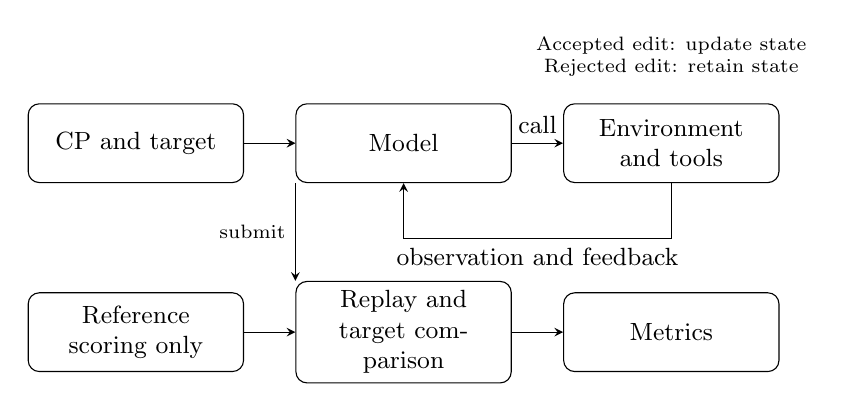
\begin{tikzpicture}[font=\small,box/.style={draw,rounded corners,align=center,text width=2.5cm,minimum height=1cm},>=stealth]
\node[box] (input) at (0,0) {CP and target};
\node[box] (model) at (3.4,0) {Model};
\node[box] (env) at (6.8,0) {Environment\\and tools};
\draw[->] (input)--(model);
\draw[->] (model)--node[above]{call}(env);
\draw[->] (env.south) -- ++(0,-.7) -| node[pos=.25,below]{observation and feedback}(model.south);
\node[align=center,font=\scriptsize] at (6.8,1.1) {Accepted edit: update state\\Rejected edit: retain state};
\node[box] (score) at (3.4,-2.4) {Replay and\\target comparison};
\node[box] (ref) at (0,-2.4) {Reference\\scoring only};
\node[box] (metrics) at (6.8,-2.4) {Metrics};
\draw[->] (model.south west)--node[left,font=\scriptsize]{submit}(score.north west);
\draw[->] (ref)--(score);
\draw[->] (score)--(metrics);
\end{tikzpicture}
\caption{Evaluation pipeline. The model edits and inspects its current construction. The reference
sequence is withheld from the model and used only for scoring.}
\label{fig:pipeline}
\end{figure}
